\subsection{Sinusoidal Forcing}
Let
\[ \ddot y + \mu \dot y + \omega_0^2 y = \sin \omega t \]
Now let us guess \(y_p = A\sin \omega t + B\cos \omega t\). Equating coefficients of \(\sin\omega t\) gives
\[ -A\omega^2 - B\mu\omega + \omega_0^2A = 1 \tag{a} \]
and equating \(\cos\omega t\) gives
\[ -B\omega^2 + A\mu\omega + \omega_0^2B = 0 \tag{b} \]
Then:
\[ (\text b) \implies A = B \frac{\omega^2 - \omega_0^2}{\mu\omega} \]
\[ (\text a) \implies A(\omega_0^2 - \omega^2) = 1 + B\mu\omega \]
So
\[ A = \frac{\omega_0^2 - \omega^2}{(\omega_0^2 - \omega^2)^2 + \mu^2\omega^2} \]
\[ B = \frac{-\mu\omega}{(\omega_0^2 - \omega^2)^2 + \mu^2\omega^2} \]
Altogether, we have
\[ y_p = \frac{1}{(\omega_0^2 - \omega^2)^2 + \mu^2\omega^2}\left[ (\omega_0^2 - \omega^2)\sin\omega t - \mu \omega \cos \omega t \right] \]
Drawing an example of this kind of particular integral in red (with the complementary function in blue), we can see the following:\medskip

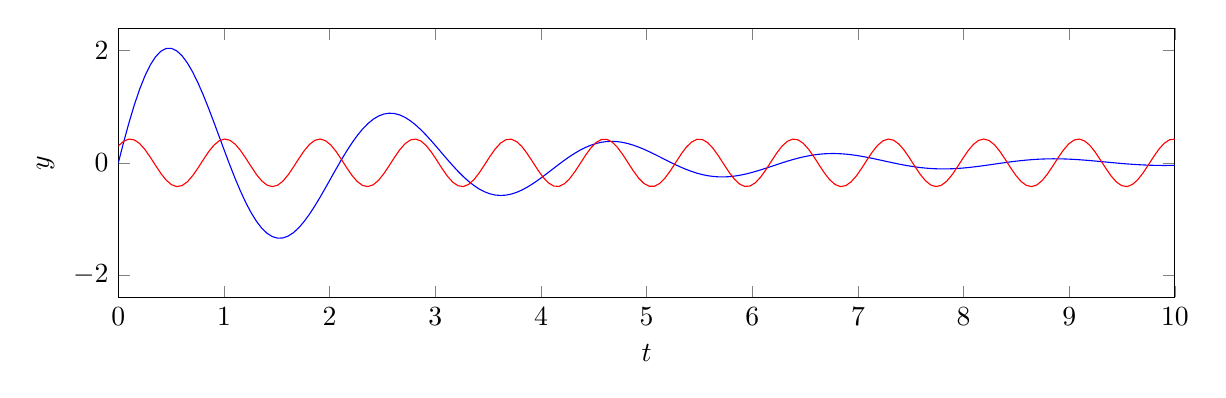
\begin{tikzpicture}
	\begin{axis}[
			%axis lines = left,
			xlabel = \(t\),
			ylabel = \(y\),% \(y = y_c + y_p\),
			width=15cm,
			height=5cm,
			xmin=0,
			xmax=10,
			ymin=-2.4,
			ymax=2.4
			%xticklabel=\empty,
			%yticklabel=\empty
		]

		\addplot [
			domain=0:10,
			samples=200,
			color=blue
		]
		{2.5*e^(-0.4*x)*sin(3*deg(x))};

		\addplot [
			domain=0:10,
			samples=200,
			color=red
		]
		{0.3*(sin(7*deg(x)) + cos(7*deg(x)))};
	\end{axis}
\end{tikzpicture}

\noindent And adding both together to form a particular solution gives:\medskip

\begin{tikzpicture}
	\begin{axis}[
			%axis lines = left,
			xlabel = \(t\),
			ylabel = \(y\),% \(y = y_c + y_p\),
			width=15cm,
			height=5cm,
			xmin=0,
			xmax=10,
			ymin=-2.4,
			ymax=2.4
			%xticklabel=\empty,
			%yticklabel=\empty
		]

		\addplot [
			domain=0:10,
			samples=200,
			color=black
		]
		{2.5*e^(-0.4*x)*sin(3*deg(x)) + 0.3*(sin(7*deg(x)) + cos(7*deg(x)))};
	\end{axis}
\end{tikzpicture}

\noindent Let us make a few comments about these forced oscillations.
\begin{itemize}
	\item The complementary function gives us the transient (short-term) response to the initial conditions.
	\item The particular integral gives the long-term response to the forcing term.
	\item In some sense, the system `forgets' about the initial conditions over time due to the damping term.
\end{itemize}

\subsection{Resonance in Undamped Systems}
What happens if \(\omega = \omega_0\)? If \(\mu \neq 0\) (i.e. it is a damped system), then
\[ \lim_{\omega \to \omega_0} y_p = \frac{-\cos\omega_0 t}{\mu\omega_0} \]
This is a finite amplitude oscillation. Note that the amplitude increases with decreasing \(\mu\), so clearly this solution has a problem at \(\mu = 0\). To work with this, we'll let
\[ \ddot y + \omega_0^2 y = \sin\omega_0 t \]
We will use detuning to get solutions for this equation. Consider instead
\[ \ddot y + \omega_0^2 y = \sin\omega t \]
where \(\omega \neq \omega_0\). We will guess that the particular integral is of the form \(y_p = C\sin\omega t\) since by inspection there cannot be any cosine terms.
\[ C(-\omega^2 + \omega_0^2) = 1 \]
\[ \therefore y_p = \frac{1}{\omega_0^2 - \omega^2}\sin\omega t \]
As the system is linear in \(y\) and its derivatives, we can freely add some multiple of the complementary function and it will remain a solution.
\[ y_p = \frac{1}{\omega_0^2 - \omega^2}\sin\omega t + A \sin\omega_0 t \]
Now let us pick \(A = \frac{-1}{\omega_0^2 - \omega^2}\), so
\[ y_p = \frac{\sin \omega t - \sin \omega_0 t}{\omega_0^2 - \omega^2} \]
Rewriting this using angle addition and subtraction identities:
\[ y_p = \frac{2}{\omega_0^2 - \omega^2}\left[ \cos\left( \frac{\omega + \omega_0}{2}t \right) \sin\left( \frac{\omega - \omega_0}{2}t \right) \right] \]
For convenience, let \(\Delta\omega \equiv \omega_0 - \omega\), and therefore \(\frac{\omega + \omega_0}{2} = w_0 - \frac{1}{2}\Delta\omega\).
\[ y_p = \frac{-2}{\Delta\omega(\omega_0 + \omega)}\left[ \cos\left( \left(\omega_0 - \frac{\Delta\omega}{2}\right)t \right) \sin\frac{\Delta\omega t}{2} \right] \]
In the following diagram, \(y_p\) is drawn in blue, with the sine term (in red) acting as an envelope for the higher-frequency cosine term. The phenomenon visible here is known as `beating', as an oscillator with a fundamental frequency slightly different to the forcing frequency will begin oscillating then stop, and repeat this cycle.\medskip

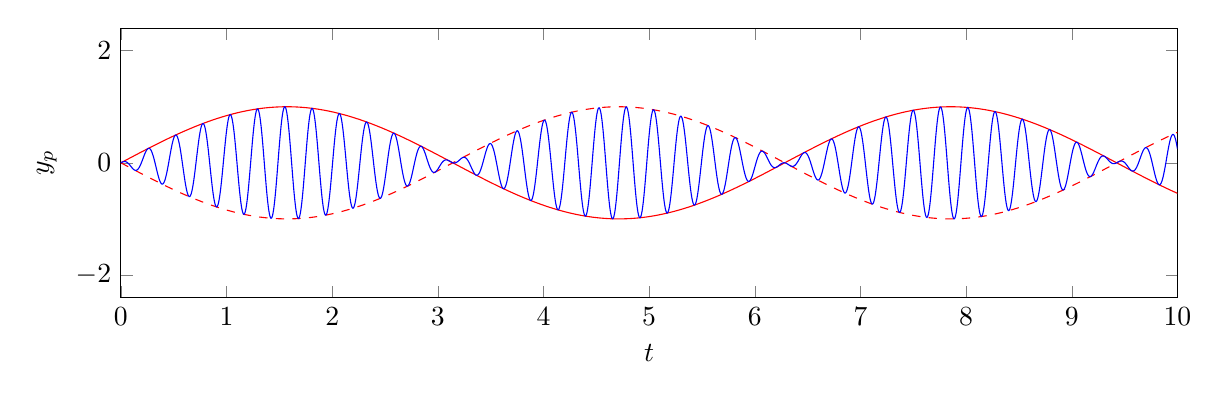
\begin{tikzpicture}
	\begin{axis}[
			%axis lines = left,
			xlabel = \(t\),
			ylabel = \(y_p\),% \(y = y_c + y_p\),
			width=15cm,
			height=5cm,
			xmin=0,
			xmax=10,
			ymin=-2.4,
			ymax=2.4
			%xticklabel=\empty,
			%yticklabel=\empty
		]

		\addplot [
			domain=0:10,
			samples=200,
			color=red
		]
		{sin(deg(x))};
		\addplot [
			dashed,
			domain=0:10,
			samples=200,
			color=red
		]
		{-sin(deg(x))};

		\addplot [
			domain=0:10,
			samples=2000,
			color=blue
		]
		{cos(24.3*deg(x))*sin(deg(x))};
	\end{axis}
\end{tikzpicture}

\noindent As we reduce \(\Delta\omega\) to zero, we have
\[ \lim_{\Delta\omega\to 0} \sin\left(\frac{\Delta\omega}{2}t\right) \approx \frac{\Delta\omega}{2}t \]
So
\begin{align*}
	\lim_{\Delta\omega\to 0}
	 & \approx \frac{-2}{\Delta\omega(\omega_0 + \omega_0)} \cos(\omega_0t)\left(\frac{\Delta\omega}{2}t\right) \\
	 & \approx \frac{-2t}{\omega_0} \cos\omega_0t                                                               \\
\end{align*}
This is linear growth in amplitude over time. This increase is unbounded an in undamped system. Note that \(y_p\) takes the form of one of the complementary functions multiplied by the independent variable.

\subsection{Impulses and Point Forces}
Consider a system that experiences a sudden force, for example a car's suspension when driving over a speed bump. Let us define \(y\) to be the displacement from the undisturbed height of the suspension. Let the car's mass be \(M\). In a small finite window \(\varepsilon\) around some time \(T\), the excess force \(F\) (the forcing term) on the system is greater than zero. As \(\varepsilon\) tends to zero, the force becomes a sudden impulse. Let us model this using the equation
\[ M\ddot y = F(t) - ky - L\dot y \]
We can see that before time \(T\), \(y=0\). After this point, there is some kind of oscillation. Note that the value of \(y\) is always continuous (otherwise this would violate many laws of physics), but the derivative is not necessarily continuous at the point \(T\). Let us integrate the equation above in time from \(T - \varepsilon\) to \(T + \varepsilon\).
\begin{equation}\label{impulse1}
	\lim_{\varepsilon \to 0} \left[ M[\dot y]_{T - \varepsilon}^{T + \varepsilon} = \int_{T - \varepsilon}^{T + \varepsilon} F(t) \dd{t} - k \underbrace{\int_{T - \varepsilon}^{T + \varepsilon} y \dd{t}}_{0\text{ if \(y\) is finite}} - L\underbrace{[y]_{T - \varepsilon}^{T + \varepsilon}}_{0\text{ if \(y\) is continuous}} \right]
\end{equation}
We now can define the impulse \(I\) to be
\[ I = \lim_{\varepsilon \to 0} \int_{T - \varepsilon}^{T + \varepsilon} F(t) \dd{t} \]
Hence
\[ \eqref{impulse1} \implies I = \lim_{\varepsilon \to 0} M[\dot y]_{T - \varepsilon}^{T + \varepsilon} \]
So if the impulse is nonzero, the velocity \(\dot y\) experiences a sudden change, so it is discontinuous at \(T\). The value of this sudden change in velocity depends on the integral of the force.
